\documentclass[landscape]{article}
\usepackage[utf8]{inputenc}

\usepackage{microtype}

\usepackage{graphicx}

\usepackage{color}

\usepackage{tikz}

\usepackage{pifont}

\usepackage{fourier-orns}

\usepackage{calculator}
% Card Arena v0.1 Colors

% Character colours
\definecolor{red}{RGB}{244,56,36}
\definecolor{blue}{RGB}{36,45,140}
\definecolor{purple}{RGB}{128,0,128}
\definecolor{green}{RGB}{63,165,56}
\definecolor{orange}{RGB}{216,128,43}
\definecolor{teal}{RGB}{51,179,198}
\definecolor{yellow}{RGB}{244,226,66}
\definecolor{brown}{RGB}{145,95,39}

\definecolor{water}{RGB}{00,119,190}
\definecolor{forest}{RGB}{65,117,5}
\definecolor{city}{RGB}{181,114,4}
\usetikzlibrary{shapes}

\pgfmathsetmacro{\hexSize}{2.5}
\pgfmathsetmacro{\hexIconSize}{0.5*\hexSize}
\pgfmathsetmacro{\tinyhexSize}{0.2*\hexSize}
\pgfmathsetmacro{\tinyhexIconSize}{0.5*\tinyhexSize}
% In the pointy orientation, a hexagon has:
% width w = sin(60) * size
% The horizontal distance between adjacent hexagon centers is w.	
\pgfmathsetmacro{\hdist}{sin(60)*\hexSize}

\tikzset{
	hexa/.style= {
		shape=regular polygon,
		regular polygon sides=6,
		minimum size=\hexSize cm, draw,
		inner sep=0,anchor=south,
		fill=lightgray!80!white,
		rotate=30 % looks quite interesting without this
	}
}
\tikzset{
	flathexa/.style= {
		shape=regular polygon,
		regular polygon sides=6,
		minimum size=\hexSize cm, draw,
		inner sep=0,anchor=south,
		fill=lightgray!80!white
		% rotate=30 % looks quite interesting without this
	}
}
\tikzset{
	tinyhexa/.style= {
		shape=regular polygon,
		regular polygon sides=6,
		minimum size=\tinyhexSize cm, draw,
		inner sep=0,anchor=south,
		fill=lightgray!80!white
		% rotate=30 % looks quite interesting without this
	}
}

\begin{document}
\begin{center}
\pagestyle{empty}

%%
%% Small Planet
%%
\begin{tikzpicture}
\pgfmathsetmacro{\boardWidthHexes}{2}
\pgfmathsetmacro{\temp}{\boardWidthHexes-1}
% bottom rows
\foreach \j in {0,...,\boardWidthHexes}{%
	\pgfmathsetmacro\end{\boardWidthHexes+\j}
	\foreach \i in {0,...,\end}{%
		\node[hexa] at ( { (\i-(\j-(\boardWidthHexes-2))/2) * \hdist }, { \j * (0.75*\hexSize) } ) {};
	}
}

% top rows
\foreach \j in {0,...,\temp}{%
	\pgfmathsetmacro\end{2*\boardWidthHexes-1-\j}
	\foreach \i in {0,...,\end}{%
		\node[hexa] at ( { (\i+(\j-1)/2) * \hdist }, { (\boardWidthHexes+1+\j) * (0.75*\hexSize) } ) {};
	}
}
\end{tikzpicture}

%%
%% Larger Planet
%%
\begin{tikzpicture}
% bottom rows
\pgfmathsetmacro{\boardWidthHexes}{3}
\pgfmathsetmacro{\temp}{\boardWidthHexes-1}
\foreach \j in {0,...,\boardWidthHexes}{%
	\pgfmathsetmacro\end{\boardWidthHexes+\j}
	\foreach \i in {0,...,\end}{%
		\node[hexa] at ( { (\i-(\j-(\boardWidthHexes-2))/2) * \hdist }, { \j * (0.75*\hexSize) } ) {};
	}
}

% top rows
\foreach \j in {0,...,\temp}{%
	\pgfmathsetmacro\end{2*\boardWidthHexes-1-\j}
	\foreach \i in {0,...,\end}{%
		\node[hexa] at ( { (\i+(\j-1)/2) * \hdist }, { (\boardWidthHexes+1+\j) * (0.75*\hexSize) } ) {};
	}
}
\end{tikzpicture}


%%
%% Terraforming Track
%%
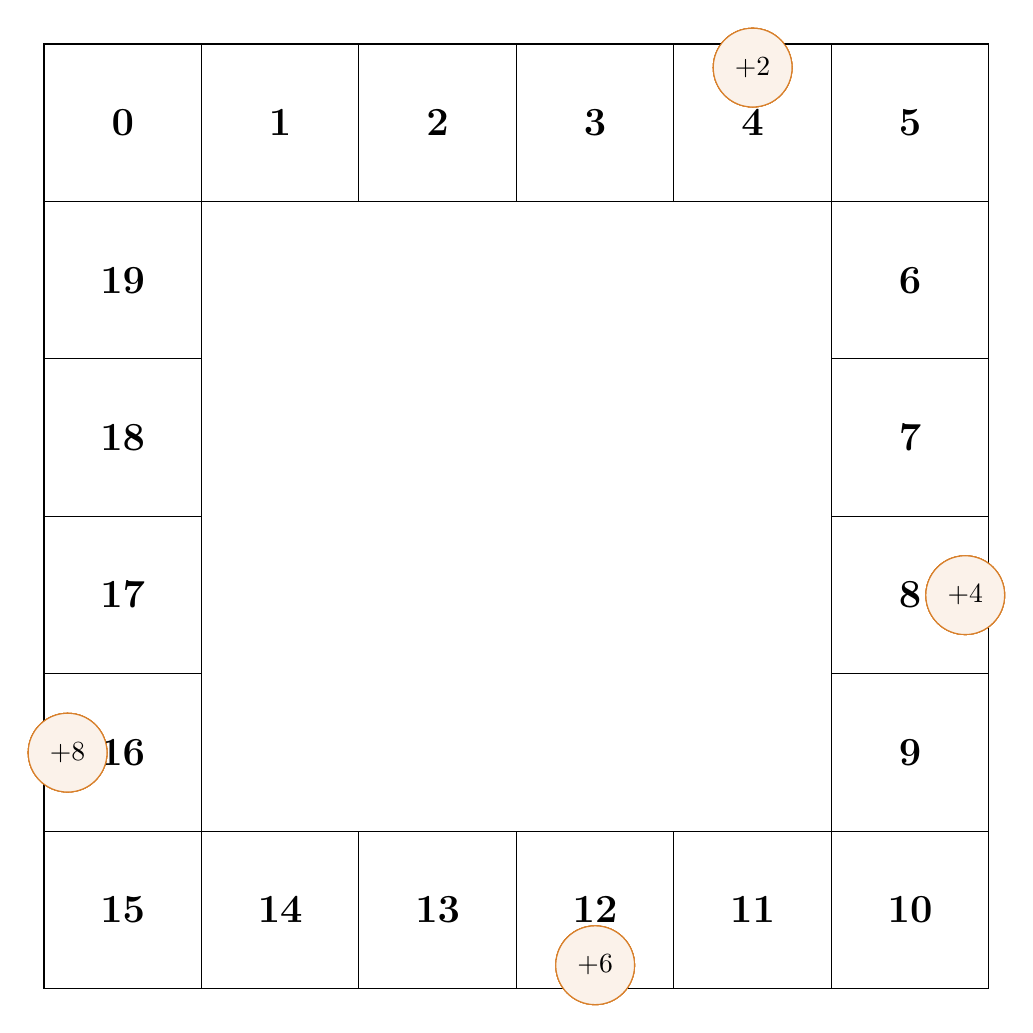
\begin{tikzpicture}
\pgfmathsetmacro{\spacesperrow}{4}
\pgfmathsetmacro{\scorespacesize}{2}
\foreach \j in {0,...,\spacesperrow}{%
	\draw[black] (\j*\scorespacesize,0) rectangle (\j*\scorespacesize+\scorespacesize,\scorespacesize);
	\filldraw[orange,fill=white!90!orange] (4.5*\scorespacesize, 0.85*\scorespacesize) circle (0.5 cm);
	\node at (4.5*\scorespacesize,0.85*\scorespacesize) {+2};
	\node at (\j*\scorespacesize+0.5*\scorespacesize,0.5*\scorespacesize) {\Large{\textbf \j}};
	
	\draw[black] (\spacesperrow*\scorespacesize+\scorespacesize,-\j*\scorespacesize+\scorespacesize) rectangle (\spacesperrow*\scorespacesize+2*\scorespacesize,-\j*\scorespacesize);
	\filldraw[orange,fill=white!90!orange] (5.5*\scorespacesize+0.35*\scorespacesize,-2.5*\scorespacesize) circle (0.5 cm);
	\node at (5.5*\scorespacesize+0.35*\scorespacesize,-2.5*\scorespacesize) {+4};
	\pgfmathtruncatemacro{\rightrow}{\j+\spacesperrow+1}
	\node at (5.5*\scorespacesize,0.5*\scorespacesize-\j*\scorespacesize) {\Large{\textbf \rightrow}};
	
	\draw[black] (\j*\scorespacesize+\scorespacesize,-\spacesperrow*\scorespacesize) rectangle (\j*\scorespacesize+2*\scorespacesize,-\spacesperrow*\scorespacesize-\scorespacesize);
	\filldraw[orange,fill=white!90!orange] (3.5*\scorespacesize,-\spacesperrow*\scorespacesize-0.85*\scorespacesize) circle (0.5 cm);
	\node at (3.5*\scorespacesize,-\spacesperrow*\scorespacesize-0.85*\scorespacesize) {+6};
	\pgfmathtruncatemacro{\bottomrow}{3*\spacesperrow+2-\j}
	\node at (\j*\scorespacesize+1.5*\scorespacesize,-\spacesperrow*\scorespacesize-0.5*\scorespacesize) {\Large{\textbf \bottomrow}};
	
	\draw[black] (0,-\j*\scorespacesize) rectangle (\scorespacesize,-\j*\scorespacesize-\scorespacesize);
	\filldraw[orange,fill=white!90!orange] (0.15*\scorespacesize,-3.5*\scorespacesize) circle (0.5 cm);
	\node at (0.15*\scorespacesize,-3.5*\scorespacesize) {+8};
	\pgfmathtruncatemacro{\leftrow}{4*\spacesperrow+3-\j}
	\node at (0.5*\scorespacesize,-\j*\scorespacesize-0.5*\scorespacesize) {\Large{\textbf \leftrow}};
}
\end{tikzpicture}

\end{center}
\end{document}
